\section{Supplementary Results}
\label{sec:supplementary-results}

\subsection{HLA-stratified Attribution Patterns}

The paired positional analysis in the main manuscript identifies P2, P3, and P9 as the most influential positions. Supplementary Figure~\ref{fig:shap-hla-motifs} further shows that this positional importance is not explained by one pooled residue pattern. For HLA-A*02:01, L, P, and Y at P2 and V, L, and Y at P9 receive positive contrasts, whereas HLA-A*24:02 and HLA-B*07:02 exhibit different residue--position structures. Each panel still combines tissues, source studies, proteins, and observational sampling; the maps therefore describe allele-associated dependence of the fitted model rather than a causal biochemical mechanism.

\begin{figure*}[t]
\centering
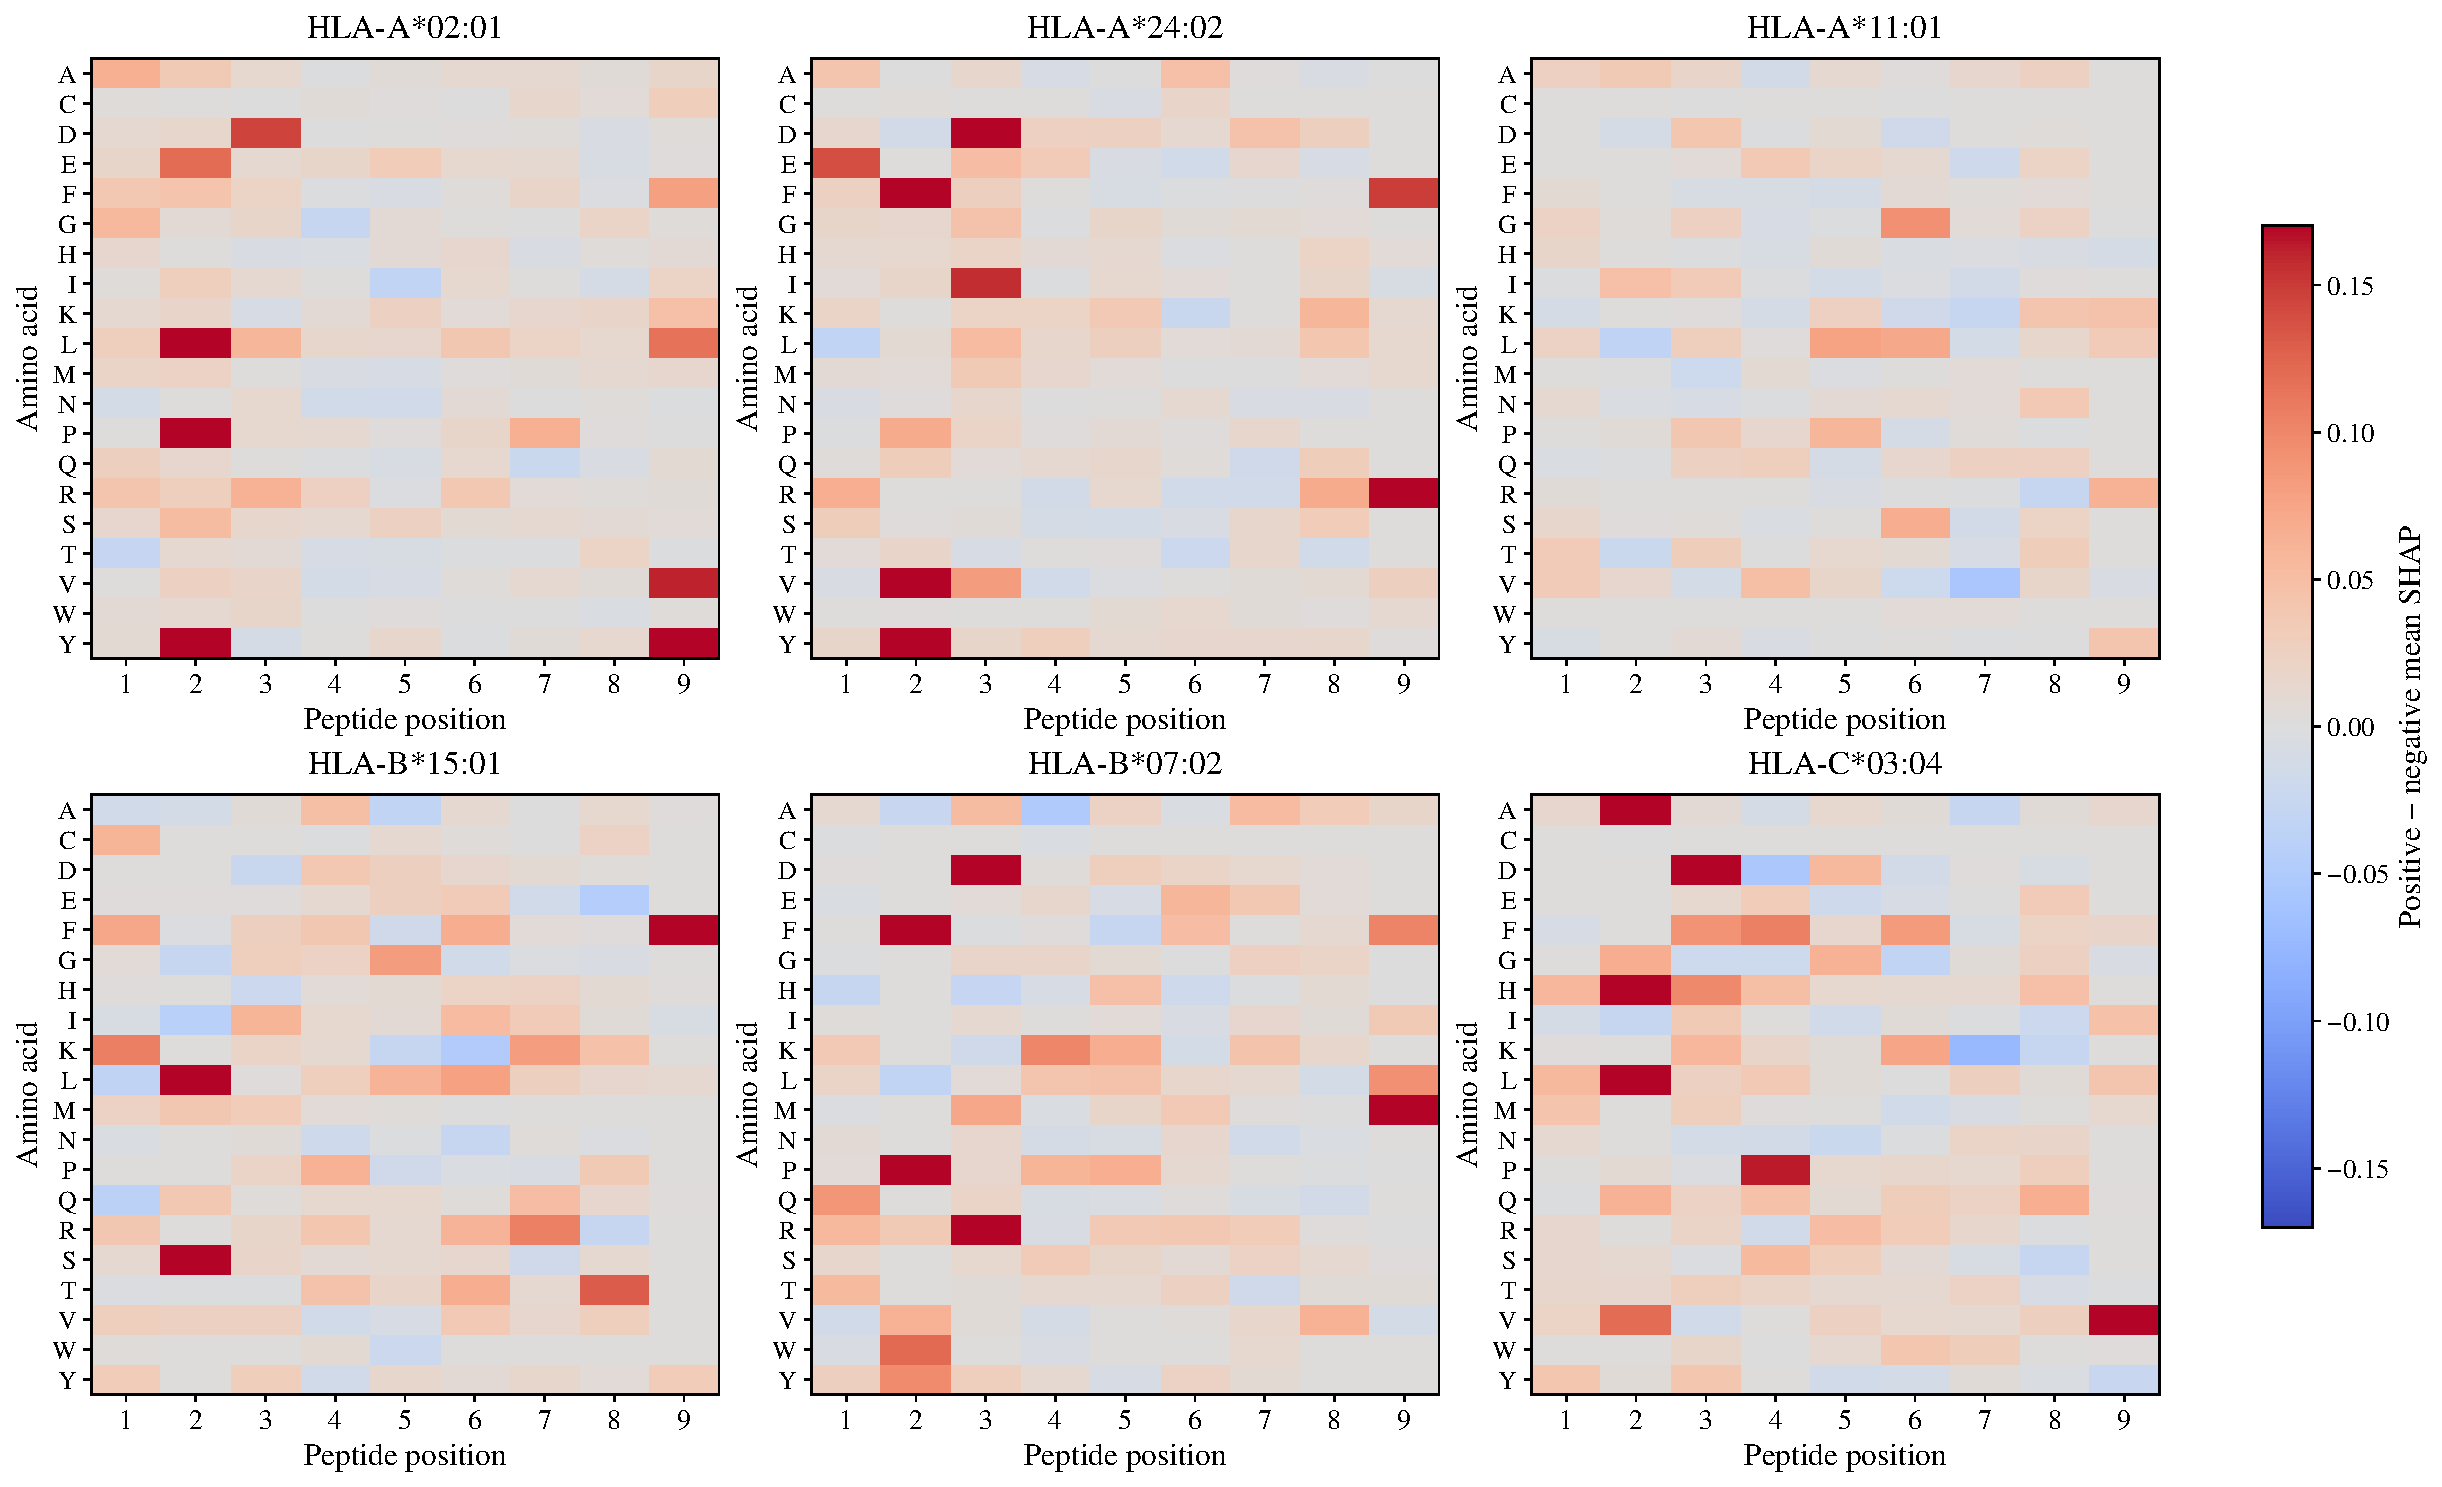
\includegraphics[width=0.98\textwidth]{figures/figure9_hla_shap_motifs.pdf}
\caption{HLA-stratified residue--position attribution maps for six well-represented Human alleles. Each cell is the mean branch-consensus attribution among recorded-positive rows minus that among occurrence-matched pseudo-negative rows for one amino acid and peptide position, aggregated across the three final-training seeds and the represented tissue--HLA tasks. Red indicates that the fitted branches associate that residue--position cell more strongly with the recorded-positive label; blue indicates the reverse. Blank-looking neutral cells are near zero, not missing measurements. Shared color limits permit visual comparison across panels. The maps describe model dependence conditional on task-specific empirical backgrounds and do not establish causal binding or antigen-processing effects.}
\label{fig:shap-hla-motifs}
\end{figure*}
\FloatBarrier

\subsection{Counterfactual Same-HLA Tissue Analysis}

The same-HLA counterfactual analysis fixes peptide, HLA, position, and substitution while changing the represented tissue task. Tissue dispersion exceeds training-seed dispersion for all 28 multi-tissue human HLA alleles, with peptide-bootstrap intervals above zero. P2, P3, and P9 have the largest pooled tissue dispersion (0.3074, 0.1920, and 0.1798). Supplementary Figure~\ref{fig:cross-tissue-ism} shows both the allele-level dispersion ratios and a representative HLA-A*02:01 tissue perturbation fingerprint. These results support fitted-model tissue conditioning but do not identify a causal antigen-processing mechanism.

\begin{figure*}[t]
\centering
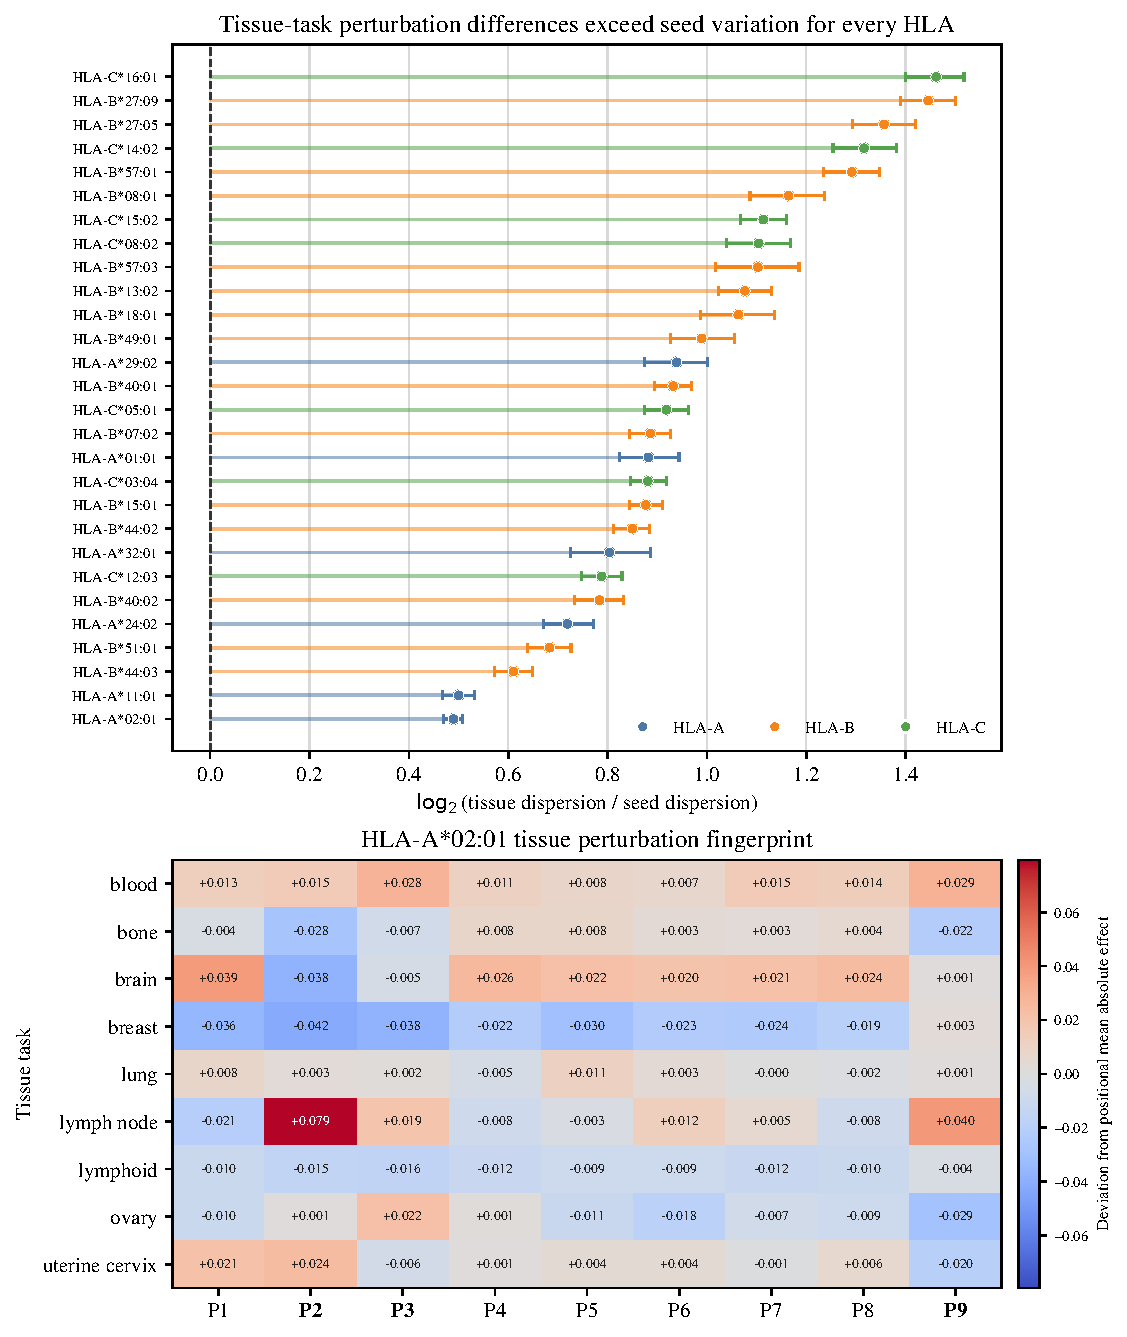
\includegraphics[width=0.88\textwidth]{figures/figure11_cross_tissue_ism.pdf}
\caption{Counterfactual same-HLA comparison of single-residue perturbation effects across Human tissue tasks. Each fixed peptide, position and substitution is scored under every represented tissue task for the same HLA. (a) HLA-level $\log_2$(tissue/seed) dispersion ratios for the final rank-fusion perturbation effect: dots are point estimates, horizontal bars are peptide-bootstrap 95\% intervals and colour denotes HLA locus; the dashed line marks equal tissue and seed dispersion. (b) A representative HLA-A*02:01 tissue perturbation fingerprint. Each cell is the three-seed mean absolute rank-fusion effect at one peptide position in one annotated tissue task, centred by the allele's across-tissue mean for that position. Red and blue denote above- and below-baseline sensitivity; P2, P3 and P9 are emphasized. These contrasts establish fitted-model task dependence under fixed peptide and HLA inputs; they do not identify a causal tissue-processing mechanism.}
\label{fig:cross-tissue-ism}
\end{figure*}
\FloatBarrier

\subsection{Detailed Tissue and Allele Heterogeneity}

Performance varies across the 77 Human tasks. The lowest individual task is brain--HLA-A*11:01 (AUROC 0.6077), whereas the highest is breast--HLA-A*02:01 (0.9640). Supplementary Table~\ref{tab:human-tissue-extremes} reports the corresponding tissue-level summaries. These values are descriptive because tissues differ in HLA inventory, source studies, peptide composition, and training coverage.

\begin{table*}[t]
\centering
\caption{Human tissue-level fixed-test performance of tuned TissuePMHC on the occurrence-matched data. The table describes heterogeneity rather than a controlled biological tissue ranking. Each of the 77 tasks is first averaged over the same three seeds; tissue means then weight the available HLA tasks equally. Task counts expose the unequal HLA inventory across tissues. Tissues are ordered by AUROC from top to bottom in the left block and then the right block; the blank source label is reported as ``NA/unspecified.''}
\label{tab:human-tissue-extremes}
\footnotesize
\begin{tabularx}{\textwidth}{>{\raggedright\arraybackslash}Xrrr>{\raggedright\arraybackslash}Xrrr}
\toprule
Tissue & Tasks & AUROC & AUPRC & Tissue & Tasks & AUROC & AUPRC \\
\midrule
Brain & 4 & 0.7314 & 0.7393 & Blood & 26 & 0.8265 & 0.8345 \\
NA/unspecified & 1 & 0.7384 & 0.7261 & Uterine cervix & 5 & 0.8328 & 0.8262 \\
Thymus & 1 & 0.7407 & 0.7548 & Bone & 1 & 0.8627 & 0.8762 \\
Lung & 7 & 0.7476 & 0.7417 & Lymph node & 5 & 0.8737 & 0.8583 \\
Spleen & 1 & 0.7765 & 0.7834 & Kidney & 1 & 0.8769 & 0.9003 \\
Lymphoid & 23 & 0.8129 & 0.8032 & Breast & 1 & 0.9640 & 0.9657 \\
Ovary & 1 & 0.8129 & 0.8200 & & & & \\
\bottomrule
\end{tabularx}
\end{table*}

The 11 Mouse tissue--H-2 tasks span AUROC 0.5016--0.9180. Supplementary Table~\ref{tab:mouse-task-detail-new} reports all task values and the corresponding H-2-restriction means. Each restriction is represented in a different tissue subset, so the table does not estimate controlled H-2 effects.

\begin{table*}[t]
\centering
\caption{Mouse heterogeneity of tuned TissuePMHC on the occurrence-matched fixed test. \textbf{A}, All 11 tissue--H-2 task values, each averaged over the same three seeds and ordered by AUROC. \textbf{B}, Descriptive H-2-restriction means formed after the seed-level task averages, with tasks weighted equally. Task counts expose the available tissue inventory. The table describes internal heterogeneity and cannot isolate tissue or H-2 effects because the represented contexts differ.}
\label{tab:mouse-task-detail-new}
\footnotesize
\begin{minipage}[t]{0.57\textwidth}
\textbf{A. Tissue--H-2 tasks}\par\smallskip
\begin{tabularx}{\linewidth}{>{\raggedright\arraybackslash}Xlrr}
\toprule
Tissue & H-2 & AUROC & AUPRC \\
\midrule
Colon & H2-Db & 0.5016 & 0.5025 \\
Liver & H2-Db & 0.6754 & 0.6695 \\
Skin & H2-Kb & 0.7821 & 0.8124 \\
Liver & H2-Kb & 0.7999 & 0.8186 \\
Spleen & H2-Kb & 0.8461 & 0.8524 \\
Spleen & H2-Kd & 0.8693 & 0.8676 \\
Skin & H2-Kk & 0.8760 & 0.8920 \\
Liver & H2-Kk & 0.9113 & 0.9126 \\
Spleen & H2-Kk & 0.9161 & 0.9220 \\
Liver & H2-Kd & 0.9180 & 0.9137 \\
Skin & H2-Kd & 0.9180 & 0.9440 \\
\bottomrule
\end{tabularx}
\end{minipage}
\hfill
\begin{minipage}[t]{0.35\textwidth}
\textbf{B. H-2 restriction groups}\par\smallskip
\centering
\begin{tabular}{lrrr}
\toprule
H-2 restriction & Tasks & AUROC & AUPRC \\
\midrule
H2-Db & 2 & 0.5885 & 0.5860 \\
H2-Kb & 3 & 0.8094 & 0.8278 \\
H2-Kd & 3 & 0.9018 & 0.9085 \\
H2-Kk & 3 & 0.9011 & 0.9089 \\
\bottomrule
\end{tabular}
\end{minipage}
\end{table*}

Human performance is also heterogeneous across HLA loci and four-digit typings. Supplementary Table~\ref{tab:human-hla-locus} reports the five lowest and five highest allele means. Unequal tissue and training inventories prevent interpretation as a controlled allele ranking.

\begin{center}
\begin{minipage}{\columnwidth}
\captionof{table}{Lowest and highest Human four-digit HLA typings by mean fixed-test AUROC of tuned TissuePMHC. Each task is first averaged over the same three seeds on the occurrence-matched fixed test; allele means then weight the represented tissue--HLA tasks equally. Typings are selected solely by AUROC, five from each tail, while AUPRC is shown as a secondary metric. Task counts expose unequal tissue coverage, so the table is a descriptive extreme-value summary rather than a controlled allele ranking.}
\label{tab:human-hla-locus}
\centering
\scriptsize
\begin{tabularx}{\columnwidth}{lXrrr}
\toprule
Group & HLA typing & Tasks & AUROC & AUPRC \\
\midrule
Lowest & HLA-A*29:02 & 2 & 0.6500 & 0.6404 \\
Lowest & HLA-A*11:01 & 3 & 0.6550 & 0.6468 \\
Lowest & HLA-B*44:03 & 3 & 0.7036 & 0.6999 \\
Lowest & HLA-B*49:01 & 2 & 0.7296 & 0.7105 \\
Lowest & HLA-B*40:02 & 3 & 0.7442 & 0.7178 \\
\midrule
Highest & HLA-C*16:01 & 2 & 0.9351 & 0.9312 \\
Highest & HLA-B*27:09 & 2 & 0.9143 & 0.9176 \\
Highest & HLA-B*27:05 & 2 & 0.9120 & 0.9082 \\
Highest & HLA-C*14:02 & 2 & 0.9119 & 0.9177 \\
Highest & HLA-C*05:01 & 3 & 0.9010 & 0.8968 \\
\bottomrule
\end{tabularx}
\end{minipage}
\end{center}

Training-only tuning increases mean task AUROC by 0.0054 in Human and 0.0489 in Mouse. Supplementary Figure~\ref{fig:tuning-delta-by-species} reports the complete task-wise distributions, bootstrap intervals, and paired tests. These statistics describe the fixed task inventories rather than independent biological samples.

\begin{figure*}[t]
\centering

\includegraphics[width=0.90\textwidth]{figures/figure7_tuned_vs_untuned_task_deltas.pdf}
\caption{Task-wise change in fixed-test AUROC after training-only hyperparameter tuning. Each point is the difference between tuned and untuned TissuePMHC after first averaging the same task over seeds; positive values favor the tuned configuration. Open diamonds show the mean change, and horizontal bars show 95\% intervals from 10,000 bootstrap resamples of complete tasks. Two-sided paired Wilcoxon signed-rank tests were performed separately for Human and Mouse, then adjusted together by Holm's method (Human: 77 tasks, mean +0.0054, 54 improved, adjusted $p=0.0060$; Mouse: 11 tasks, mean +0.0489, 10 improved, adjusted $p=0.0039$). The intervals and tests describe this internal fixed-test task inventory and are not biological-replicate or cohort-level inference.}
\label{fig:tuning-delta-by-species}
\end{figure*}

\subsection{Detailed Tissue-independent Neural Control}

Removing tissue identity while retaining peptide and MHC information creates an intentionally ambiguous prediction problem: the same peptide--MHC query may be positive in one tissue and a pseudo-negative in another. Supplementary Table~\ref{tab:tissue-blind-conflict-audit} quantifies this label structure. Among queries represented by multiple tissue-specific rows, 95.18--99.04\% contain both labels across the species and partition summaries.

\begin{table}[H]
\centering
\caption{Deterministic label-conflict audit for controls without tissue information. Queries are defined by peptide sequence and MHC restriction. ``One'' and ``multiple'' count queries with one or multiple retained labels; conflicting queries contain both labels. Conflict percentages use multiple-label queries as the denominator.}
\label{tab:tissue-blind-conflict-audit}
\fontsize{5.9}{6.8}\selectfont
\setlength{\tabcolsep}{1.7pt}
\renewcommand{\arraystretch}{1.05}
\begin{tabularx}{\columnwidth}{@{}>{\raggedright\arraybackslash}Xrrrrrr@{}}
\toprule
\multicolumn{7}{@{}l}{\textbf{Human benchmark}} \\
Partition & Rows & \shortstack{Unique\\queries} & One & Multiple & Conflict & \% \\
\midrule
Training pool & 42,978 & 27,063 & 12,572 & 14,491 & 14,168 & 97.77 \\
Fixed test & 7,700 & 7,012 & 6,327 & 685 & 652 & 95.18 \\
Complete benchmark & 50,678 & 29,662 & 10,441 & 19,221 & 18,882 & 98.24 \\
\midrule
\multicolumn{7}{@{}l}{\textbf{Mouse benchmark}} \\
Partition & Rows & \shortstack{Unique\\queries} & One & Multiple & Conflict & \% \\
\midrule
Training pool & 4,178 & 2,934 & 1,735 & 1,199 & 1,175 & 98.00 \\
Fixed test & 1,100 & 996 & 892 & 104 & 103 & 99.04 \\
Complete benchmark & 5,278 & 3,338 & 1,487 & 1,851 & 1,833 & 99.03 \\
\bottomrule
\end{tabularx}
\end{table}

Supplementary Table~\ref{tab:trainable-tissue-blind-control} reports the fitted MHC-only convolutional control. It loses 0.5211 mean task AUROC in Human and 0.6026 in Mouse and is worse than full TissuePMHC in every evaluated task. The below-random values reflect the cross-tissue label ambiguity rather than ordinary reverse generalization. Input-invariance checks confirm that identical peptide--MHC queries receive equal scores across tissues up to the prespecified numerical tolerance.

\begin{table}[H]
\centering
\caption{Trainable MHC-only control on the occurrence-matched fixed tests. AUROC and AUPRC are task-macro mean $\pm$ sample standard deviation across seeds 20260704--20260706. $\Delta$ AUROC is candidate minus full TissuePMHC after averaging each task across seeds; brackets give a 10,000-resample task-bootstrap 95\% confidence interval. W/T/L counts task-wise positive/zero/negative deltas. The exact two-sided paired Wilcoxon test is the prespecified MHC-only contrast. Identical peptide--MHC queries are constrained only by model inputs, not by post-hoc score averaging.}
\label{tab:trainable-tissue-blind-control}
\scriptsize
\setlength{\tabcolsep}{3pt}
\renewcommand{\arraystretch}{1.08}
\begin{tabularx}{\columnwidth}{@{}>{\raggedright\arraybackslash}Xrr@{}}
\toprule
\multicolumn{3}{@{}l}{\textbf{Human benchmark}} \\
Model & AUROC & AUPRC \\
\midrule
Full TissuePMHC & $0.8136\pm0.0021$ & $0.8126\pm0.0021$ \\
Trainable MHC-only CNN & $0.2925\pm0.0062$ & $0.3932\pm0.0040$ \\
\multicolumn{3}{@{}p{\columnwidth}@{}}{$\Delta$ AUROC $=-0.5211$ [95\% CI $-0.5489,-0.4927$]; W/T/L $=0/0/77$; $p=2.46\times10^{-14}$.} \\
\midrule
\multicolumn{3}{@{}l}{\textbf{Mouse benchmark}} \\
Model & AUROC & AUPRC \\
\midrule
Full TissuePMHC & $0.8194\pm0.0157$ & $0.8279\pm0.0121$ \\
Trainable MHC-only CNN & $0.2168\pm0.0052$ & $0.3686\pm0.0064$ \\
\multicolumn{3}{@{}p{\columnwidth}@{}}{$\Delta$ AUROC $=-0.6026$ [95\% CI $-0.7183,-0.4617$]; W/T/L $=0/0/11$; $p=0.0010$.} \\
\bottomrule
\end{tabularx}
\end{table}
